\documentclass{tufte-handout}


\usepackage[utf8]{inputenc}

\usepackage{graphicx} % for handling images

\usepackage{amsmath}
\usepackage{booktabs}
\usepackage{microtype}

\usepackage{pgfplots} % layout and margin handling
\pgfplotsset{width=9cm,compat=1.13}

\usepackage{booktabs}
\usepackage{tcolorbox}

\title{Applied Algorithms\newline Optional Assignment \#1}
% \author{Hugo de Brito\newline hubr@itu.dk}

\begin{document}
\thispagestyle{empty}

\maketitle


\includegraphics[width=\textwidth]{logo_en.png}

\vspace{5mm}\noindent %10mm vertical space

\begin{table}[!h]
\centering
\begin{tabular}{cc}
\multicolumn{2}{c}{Authors}                                   \\ \hline
\multicolumn{1}{c|}{\textbf{Hugo Brito}} & \textbf{René Haas} \\
\multicolumn{1}{c|}{\href{mailto:hubr@itu.dk}{hubr@itu.dk}}         & \href{mailto:renha@itu.dk}{renha@itu.dk}       \\ \hline
\end{tabular}
\end{table}

\vspace{5mm} %10mm vertical space

\section{Implement Naive, Recursive, and Strassen's Algorithm, and compare them.}

\noindent Implement the the recursive algorithm and Strassen (for example, in the same JupterLab project), and compare the results in a plot! Submit the code, your plot, and add a few (informal) sentences on your interpretation of the plots.

\section{Files}
This reports the work developed around the implementation of different algorithms for solving square matrix multiplication. The files can be found in the {\tt src} folder and they comprise of:
\begin{itemize}
    \item A Square Matrix Generator -- {\tt squareMatrixGenerator.java}
    \item The Naive Algorithm implementation -- {\tt NaiveMatrixMultiplication.java}
    \item The Recursive Algorithm implementation -- {\tt recursiveMatrixMultiplication.java}
    \item The Strassen's Algorithm implementation -- {\tt strassensMatrixMultiplication.java}
    \item A Java class created for the purpose of reporting the running times -- {\tt expMatrixMultiplication.java}
    \item A {\tt Makefile} instance created for the purpose of running the whole experiment at once
\end{itemize}

\section{Tests}
All the matrix multiplication algorithms pass all tests on Code Judge. Also, to avoid dead code and ensure correctness in the multiplication, we have implemented a method in the {\tt expMatrixMultiplication}, {\tt Arrays.deepEquals} which compares each of the values contained in each cell of the matrices and returns a {\tt boolean} value that informs of the validity of that specific calculation. Every result obtained either via the recursive or the Strassen's algorithms was compared to the one obtained via naive multiplication and returned {\tt true}, which also proves the hypothesis of all algorithms calculating correctly.\\

\section{Experiments}
\begin{tcolorbox}
\begin{itemize}
\item {\bf Question:} Is the running time of the Strassen's algorithm for Matrix Multiplication smaller than the naive and/or the recursive algorithms?
\item {\bf Performance indicators:} Running times
\item {\bf Factors:}
\begin{itemize}
  \item Input type: Matrices $A$ and $B$ of size $n$, containing pseudo-random integers ranging from $a$ to $b$
  \item Pseudo-random seed $= 42$
  \item $n = \left\{2,4,8,16,32,64,128,256,512,1024,2048,4096,8192\right\}$
  \item $[a,b] = [-100, 100]$
\end{itemize}
% \item {\bf Levels:}
\item {\bf Trials: } $10$ repetitions per $n$
% \item {\bf Design Points:}Full factorial
\item {\bf Outputs:} Running times of each of the solving algorithms
\end{itemize}
\end{tcolorbox}

% \bigskip
\noindent
We have ran the described experiment and obtained the running times. These were outputted to a file -- {\tt res01.csv} -- that can be found in the {\tt out} folder. These were plotted and we obtained the following:

\begin{figure}[h!tb]
\centering
%[width=\linewidth]
  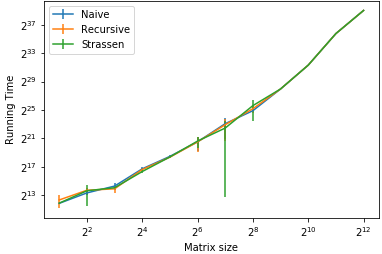
\includegraphics[scale=0.67]{out/matrixMultiplication/matrixmult.png}
  \caption{$log_2$ $log_2$ plot of the average running times (nanoseconds) vs. matrix size of the $3$ algorithms}
  \label{fig:Plot}
\end{figure}

\section{Conclusion}
Unfortunately, we could not find any significant difference in the running times between all the $3$ algorithms. We were expecting the running time of the Strassen's algorithm to be slightly better than the naive and the recursive one. Perhaps with bigger matrices the difference would be noticeable, but for now we have no way of being sure.

\end{document}